\documentclass{report}

\usepackage{amsmath,amsfonts}
\usepackage{authblk}
\usepackage{graphicx}
\usepackage{caption,subcaption}
%\usepackage{color}
%\usepackage{etoolbox}
\usepackage{float}
\usepackage{fullpage}
%\usepackage{mathtools}
\usepackage{natbib}
\usepackage[inline]{enumitem}
\usepackage{subdepth}
%\usepackage{appendix}
%\usepackage{setspace}
\usepackage{algorithm}
\usepackage{algpseudocode}
\usepackage{hyperref}

\renewcommand\thesection{\arabic{section}}
\usepackage{xspace}
\newcommand{\textcompute}{\textsf}
\newcommand{\N}{\text{N}} % Normal 
\newcommand{\R}{\textcompute{R}\xspace}
\newcommand{\IG}{\text{InvGam}}
\newcommand{\RL}{f}
\newcommand{\RLorig}{\text{RL}}
\newcommand{\logRL}{\log\RL}
\newcommand{\logRLorig}{\log\RLorig}
\newcommand{\sigssq}{\sigma_s^2}
\newcommand{\sigesq}{\sigma_e^2}
\newcommand{\sshat}{\hat\sigma^2_e,\hat\sigma^2_s}
\newcommand{\logRLss}{\logRL(\sigesq,\sigssq)}
\newcommand{\logRLssorig}{\logRLorig(\sigesq,\sigssq)}
\newcommand{\ass}{a_j\sigssq + \sigesq}
\newcommand{\abss}{a_j\sigssq + b_j\sigesq}
\newcommand{\fss}{f(\sigesq,\sigssq)\,}
%\newcommand{\mrle}{MRLE}
\newcommand{\mrle}{$\argsup\log f$}
%\newcommand{\lone}{\textbf{l}_1}
%\newcommand{\pone}{\textbf{p}_1}
%\newcommand{\ltwo}{\textbf{l}_2}
%\newcommand{\ptwo}{\textbf{p}_2}
%\newcommand{\pthree}{\textbf{p}_3}
%\newcommand{\given}{\,|\,}
\newcommand{\g}{\,|\,}
\newcommand{\maxit}{\textcompute{maxit}}
\newcommand{\argmax}{\operatornamewithlimits{argmax}}
\newcommand{\argsup}{\operatornamewithlimits{argsup}}
\newcommand*\DNA{\textsc{dna}}
\newcommand*\Let[2]{\State #1 $\gets$ #2}
\renewcommand{\bibname}{References}
\linespread{1.6}

\begin{document}

\title{Approximately Exact Calculations for Linear Mixed Models}
\author[1]{Michael Lavine}
\author[2]{Andrew Bray}
\author[3]{James Hodges}
\affil[1]{Department of Mathematics and Statistics, University of Massachusetts, Amherst, MA 01003 USA}
\affil[2]{Reed College, Portland, OR, 97202 USA}
\affil[3]{Division of Biostatistics, University of Minnesota, Minneapolis, MN, 55455 USA}

\maketitle

\begin{abstract}
This paper is about computations for linear mixed models having two variances, $\sigma^2_e$ for residuals and $\sigma^2_s$ for random effects, though the ideas can be extended to some linear mixed models having more variances.  Researchers are often interested in either the restricted (residual) likelihood $\RLorig(\sigesq,\sigssq)$ or the joint posterior $\pi(\sigesq,\sigssq\g y)$ or their logarithms.  Both $\log\RLorig$ and $\log\pi$ can be multimodal and computations often rely on either a general purpose optimization algorithm or MCMC, both of which can fail to find regions where the target function is high.  This paper presents an alternative.  Letting $f$ stand for either $\RLorig$ or $\pi$, we show how to find a box $B$ in the $(\sigesq,\sigssq)$ plane such that
\begin{enumerate}
\item all local and global maxima of $\log f$ lie within $B$;
\item $\sup_{(\sigesq,\sigssq) \in B^c} \log f(\sigesq,\sigssq) \le \sup_{(\sigesq,\sigssq) \in B} \log f(\sigesq,\sigssq) - M$ for a prespecified $M>0$; and
\item $\log f$ can be estimated to within a prespecified tolerance $\epsilon$ everywhere in $B$ with no danger of missing regions where $\log f$ is large.
\end{enumerate}
Taken together these conditions imply that the $(\sigesq,\sigssq)$ plane can be divided into two parts: $B$, where we know $\log f$ as accurately as we wish,  and $B^c$, where $\log f$ is small enough to be safely ignored.  We provide algorithms to find $B$ and to evaluate $\log f$ as accurately as desired everywhere in $B$.
\end{abstract}

\section{Introduction}
\label{sec:intro}
Linear mixed models are an important class of statistical models.  Books are written about them (e.g.\ \citealt{bryk_raudenbush:1992, verbeke&molenberghs:2000, hodges:2013, west&welch&galecki:2014}),  courses are taught about them, and they have many applications.  Typical notation, which we adopt, is
\begin{equation}
\label{eq:lmm}
	y = X\beta + Zu + \epsilon
\end{equation}
where $y$ is a vector of $n$ observations, $X$ is a known $n \times p$ matrix, $\beta$ is a vector of $p$ unknown coefficients called fixed effects, $Z$ is a known $n \times q$ matrix, $u$ is a vector of $q$ unknown coefficients called random effects, and $\epsilon$ is a vector of $n$ errors. The term ``mixed" is used when we treat $u$ as a vector of random variables, thus mixing fixed and random effects in the same model.  For linear mixed models where $u$ and $\epsilon$ are modelled as Normal, researchers are often interested in the restricted likelihood function
\begin{equation}
\label{eq:rll}
  \RLorig(\theta) = K |V(\theta)|^{-1/2}|X^tV^{-1}(\theta)X|^{-1/2}
                       \exp\left\{ -\frac{1}{2} \left(y^tV^{-1}(\theta)y -
                                                                \tilde\beta^t(\theta)X^tV^{-1}(\theta)X\tilde\beta(\theta)
                                                         \right)
                              \right\}
\end{equation}
where $K$ is an unimportant constant, $\theta$ is a vector of unknown parameters in the covariance matrices of $u$ and $\epsilon$, $V(\theta)$ is the marginal covariance matrix of $y$ implied by the covariance matrices of $u$ and $\epsilon$, and $\tilde\beta(\theta)$ is the generalized least-squares estimate of $\beta$, given $V(\theta)$.
This manuscript deals with the special case in which we adopt the model
\begin{equation*}
	\epsilon \sim \N (0, \sigma_e^2 \Sigma_e) \qquad u \sim \N (0, \sigma_s^2 \Sigma_s)
\end{equation*}
where $\Sigma_e$ and $\Sigma_s$ are known matrices, often the identity, of the appropriate sizes and $\theta \equiv (\sigma_e^2, \sigma_s^2)$, two unknown variance parameters.  The key for this manuscript is that $\theta$ contains only those two unknown variances and no others.  Examples include random intercept models (including balanced and unbalanced one-way random effect models), additive models with one penalized spline, spatial models with one intrinsic conditional autoregression (ICAR) random effect, dynamic linear models with one system-level variance, and some multiple membership models (e.g.\ \citealt{browne_etal:2001, mccaffrey_etal:2004}).  \cite{hodges:2013} examines these and other examples and explains the importance of this special case.

\cite{hodges:2013} also unifies and generalizes \cite{reich_hodges:2008} and \cite{welham_thompson:2009} to show that in our special case, and a few others, $\logRLssorig$ can be expressed as
\begin{equation}
\label{eq:reexpress}
  \logRLssorig = B - \frac{n_e}{2}\log(\sigesq) - \frac{y^t \Gamma_c \Gamma^t_c y}{2\sigesq} 
    - \frac{1}{2} \sum_{j=1}^{s_z} \left[ \log(\ass) + \frac{\hat v_j^2}{\ass}\right]
\end{equation}
where
\begin{enumerate}[label=(\arabic*)]
  \item $B$ is an unimportant known constant;
  \item $n_e$ is $n$ minus the dimension of the space spanned by the columns of $[X|Z]$;
  \item $\Gamma_c$ is $n \times n_e$ and spans the space orthogonal to $[X|Z]$
    (so $y^t \Gamma_c \Gamma^t_c y$ is the residual sum of squares);
  \item $s_z$ is the dimension of the space spanned by the columns of $Z$ not already
    in the span of the columns of $X$; and
  \item the $\{a_j\}$ and $\{\hat v_j\}$ are known constants whose derivation is in the Appendix.  All $a_j>0$.
\end{enumerate}
Thus the only unknowns are $(\sigma^2_s, \sigma^2_e)$ and $\logRLssorig$ is a function of just those two arguments.

As \cite{hodges:2013} further observes, if $\beta$ is given an improper flat prior and $\sigesq$ and $\sigssq$ are given conjugate priors --- say $\sigesq \sim \IG(\alpha_e,\beta_e)$ and $\sigssq \sim \IG(\alpha_s,\beta_s)$ --- then \begin{equation*}
  -(\alpha_e+1) \log\sigesq - \beta_e/\sigesq -(\alpha_s+1) \log\sigssq - \beta_s/\sigssq
\end{equation*}
is added to \eqref{eq:reexpress} to yield
the log posterior
\begin{equation}
\label{eq:logpost}
  \begin{split}
  \log\pi(\sigesq,\sigssq\g y) &=
  B - \frac{n_e + 2\alpha_e + 2}{2}\log(\sigesq) -
    \frac{y^t \Gamma_c \Gamma^t_c y + 2\beta_e}{2\sigesq}\\
    &\qquad\qquad - \frac{2\alpha_s + 2} {2}\log(\sigssq) - \frac{2\beta_s}{2\sigssq}
    - \frac{1}{2} \sum_{j=1}^{s_z} \left[ \log(\ass) + \frac{\hat v_j^2}{\ass}\right].
  \end{split}
\end{equation}
Equations~\eqref{eq:reexpress} and~\eqref{eq:logpost} can both be written as a sum of multiples of logs and inverses of linear combinations $\abss$, as in \eqref{eq:sum}, where the summands with $j=s_z+1$ and $j=s_z+2$ are for the terms involving only $\sigesq$ and $\sigssq$, respectively, and where we have dropped the irrelevant constant $B$.  I.e.,
\begin{equation}
\label{eq:sum}
  \logRLss = -\frac{1}{2} \sum_{j=1}^{s_z+2}\left[ c_j \log(\abss) + \frac{d_j}{\abss}\right]
\end{equation}
where
\begin{itemize}[label=---]
\item for $j = 1, \dots, s_z$,
  \begin{align*}
    a_j &> 0\ \text{and is derived in the Appendix}\\
    b_j &=1\\
    c_j &=1\\
    d_j &= \hat v_j^2\ \text{is a known function of $y$ derived in the Appendix}
  \end{align*}
\item for $j = s_z +1$,
  \begin{align*}
    a_j &= 0\\
    b_j &= 1\\
    c_j &= \begin{cases}
                 n_e & \text{for $\logRLorig$ in \eqref{eq:reexpress}}\\
                 n_e + 2\alpha_e + 2 & \text{for the $\log$ posterior in \eqref{eq:logpost}}
              \end{cases}\\
    d_j &= \begin{cases}
                 y^t \Gamma_c \Gamma^t_c y & \text{for $\logRLorig$ in \eqref{eq:reexpress}}\\
                 y^t \Gamma_c \Gamma^t_c y + 2\beta_e & \text{for the $\log$ posterior in \eqref{eq:logpost}}
              \end{cases}
  \end{align*}
\item for $j = s_z+2$,
  \begin{align*}
    a_j &= 1\\
    b_j &= 0\\
    c_j &= \begin{cases}
      0 & \text{for $\logRLorig$ in \eqref{eq:reexpress}}\\
      2 \alpha_s + 2 & \text{for the $\log$ posterior in \eqref{eq:logpost}}
    \end{cases}\\
    d_j &= \begin{cases}
      0 & \text{for $\logRLorig$ in \eqref{eq:reexpress}}\\
      2 \beta_s & \text{for the $\log$ posterior in \eqref{eq:logpost}}.
    \end{cases}
  \end{align*}
\end{itemize}
Our derivation proceeds from \eqref{eq:sum}.  We use $f$ to denote the target function generically, either $\RLorig(\sigesq,\sigssq)$ or $\pi(\sigesq,\sigssq\g y)$.  When the target function is $\RLorig(\sigesq,\sigssq)$, $c_{s_z+2} = d_{s_z+2} = 0$ and the upper limit of the sum in \eqref{eq:sum} is effectively $s_z+1$.

It is known (e.g.\ \citealt{henn&hodges:2014}) that $\logRLss$
can have multiple maxima,
though the incidence of multiple maxima is unknown.  Multi-modal posterior distributions arise readily from conflict between the likelihood and prior;  \cite{Liu&Hodges:2003} explores an important such conflict in detail and \cite{wakefield:1998} gives a naturally-occurring example explored further in \cite{henn&hodges:2014}.  Multiple maxima in restricted likelihoods have received far less attention and any statement about their incidence would be speculation.  To our knowledge, two naturally-occurring cases have been reported, in \cite{welham_thompson:2009} and \cite{reiss_etal:2014};  \cite{henn&hodges:2014} report an artificial case and give a recipe for manufacturing examples.  

As for numerical optimizers, it is known that existing general purpose algorithms for linear mixed models may fail to find all of the local maxima of $\logRLss$, as shown by examples in \cite{hodges:2013}, \cite{henn&hodges:2014}, and elsewhere.  \cite{mullen:2014} examines 18 optimization functions available in \R, tests them on 48 objective functions (admittedly more complicated than $\logRLss$) and finds that even the best of them fail in over 10\% of the cases.  \cite{henn&hodges:2014} examine conditions under which multiple maxima occur in posterior densities and conclude ``\dots second maxima in posterior distributions therefore may be more common than reports in the literature would suggest."  Thus, failure to find local and global maxima may be common, though with available tools it is extremely laborious to determine whether multiple maxima are present and where they are.

Our view is that it is important to find regions where $f$ or $\log f$ is large relative to its maximum regardless of whether those regions contain local maxima.  Points with large $\logRLss$ are those that describe the data, or possibly  prior information, well, at least compared to points with low $\logRLss$.  If $f$ or $\log f$ is relatively flat and large over a region, it matters little whether the region contains small bumps that are, technically, local maxima.  A good analysis should strive to find all  points with large $\logRL$.  Therefore, the purpose of this paper is to introduce an algorithm that will, in finite time, divide the $(\sigesq,\sigssq)$ plane into two parts: one where we know $\logRL$ is small relative to its maximum and another where we know $\logRL$ to within a pre-specified $\epsilon$ (hence the term ``approximately exact'').  The algorithm can also be used to find $(\sshat) \equiv \argsup_{\sigesq, \sigssq}\logRLss$  (typically either the maximum restricted log likelihood estimate or the maximum \textit{a posteriori} estimate), to within a pre-specified tolerance without fear of missing regions of high $f$ or $\logRL$.

The technique relies on the partial derivatives of $\logRLss$.  Analysis of the partial derivatives allows us to satisfy two desiderata.
\begin{description}
\item[D1] For any prespecified constant $M>0$ we can find a box $B$, a rectangle in the first quadrant of the $(\sigssq, \sigesq)$ plane whose sides are parallel to the axes, such that
\begin{equation}
\label{eq:boundingbox}
	\text{all local maxima are in $B$} \qquad \text{and} \qquad \sup_{(\sigesq, \sigssq) \in B^c} \logRLss \le \logRL(\sshat) - M.
\end{equation}
In practice we will take $M$ large enough to interpret (\ref{eq:boundingbox}) as meaning that we can restrict attention to $B$ because values of $(\sigesq, \sigssq) \in B^c$ have $\logRLss$ too low to be of further interest.

\item[D2] For any box $b$ with sides parallel to the axes we can quickly compute lower and upper bounds $(L^b,U^b)$ satisfying
\begin{equation*}
  L^b \le \inf_{(\sigesq, \sigssq) \in b}\logRLss \qquad\text{and}\qquad
  U^b \ge \sup_{(\sigesq, \sigssq) \in b}\logRLss
\end{equation*}
and such that $U^b-L^b \rightarrow 0$ as $b$ shrinks.  Therefore, partitioning the box $B$ from \textbf{D1} allows us to know $\logRLss$ everywhere in $B$ to within a pre-specified tolerance and also to locate $\argsup\logRL$ to within a pre-specified tolerance without fear of missing regions of high $\logRL$.
\end{description}
\textbf{D1} and \textbf{D2} allow us to divide the $(\sigesq,\sigssq)$ plane into two parts: one where $\logRL$ is at least $M$ below its maximum and another where we know $\logRL$ to within a pre-specified $\epsilon$.  The next section shows how the partial derivatives are used to satisfy \textbf{D1} and \textbf{D2}: the partial derivatives determine lines in the $(\sigesq,\sigssq)$ plane; those lines determine a box $B_1$ containing all local maxima and a larger box $B \supset B_1$ satisfying \textbf{D1}; and those lines also determine upper and lower bounds on $\logRL$ within any box $b$.

\section{Satisfying the Desiderata}
\subsection{Partial Derivatives Determine Lines}
\label{subsec:lines}
The partial derivatives of $\logRLss$ can be calculated from (\ref{eq:sum}):
\begin{subequations}
\label{eq:partials}
\begin{equation}
\label{eq:drlds}
  \frac{\partial\logRLss}{\partial\sigssq}
  = -\frac{1}{2} \sum_{j=1}^{s_z+2}
        \left[ \frac{a_jc_j}{\abss} - \frac{a_j d_j}{(\abss)^2} \right]
        = -\frac{1}{2} \sum_{j=1}^{s_z+2}
            \frac{a_j \left( a_jc_j\sigssq + b_jc_j\sigesq  - d_j\right)}{(\abss)^2}\\
\end{equation}
and
\begin{equation}\label{eq:drlde}
  \frac{\partial\logRLss}{\partial\sigesq} =
    -\frac{1}{2} \sum_{j=1}^{s_z+2} \left[ \frac{b_jc_j}{\abss} - \frac{b_j d_j}{(\abss)^2} \right]
    = - \frac{1}{2} \sum_{j=1}^{s_z+2}
         \frac{b_j \left( a_jc_j\sigssq + b_jc_j\sigesq  - d_j\right)}{(\abss)^2}.
\end{equation}
\end{subequations}

We work with one term in (\ref{eq:partials})'s summations at a time; that is, one $j$ at a time.  For $j=1, \dots, s_z$, the $j$'th terms in (\ref{eq:partials}) differ  by a multiplicative constant $a_j/b_j = a_j$; they have the same sign as each other and the same sign as $(a_jc_j\sigssq + b_jc_j\sigesq  - d_j) = (a_j\sigssq + \sigesq  - d_j)$, which determines a line $\sigssq = d_j/a_j - \sigesq/a_j$ --- call it the $j$'th line --- in the first quadrant of the $(\sigssq,\sigesq)$ plane.  The $j$'th line has positive intercept $ d_j/a_j$ and negative slope $-1/a_j$.  For $j=s_z+1$, $a_j=0$, so $\eqref{eq:drlds} = 0$ and \eqref{eq:partials} determines a vertical line at $\sigesq = \sigma_e^{2*} \equiv d_{s_z+1} / c_{s_z+1}$.  For $j=s_z+2$,  $b_j=0$, so $\eqref{eq:drlde} = 0$ and, if the target function is \eqref{eq:logpost}, \eqref{eq:partials} determines a horizontal line at $\sigssq = \sigma_s^{2*} \equiv d_{s_z+2} / c_{s_z+2}$, while if the target function is \eqref{eq:reexpress}, $c_{s_z+2} = d_{s_z+2} = 0$; the term for $j=s_z+2$ effectively vanishes and there is no horizontal line.

For all $j$, both partial derivatives of the $j$'th term are nonnegative below or to the left of the $j$'th line, 0 on the line, and nonpositive above or to the right of the line, as indicated in Figure~\ref{fig:oneline}.  The $j$'th term is constant on the $j$'th line and attains its maximum there.

\begin{figure}[h]
	\centering
	\includegraphics[width=.5\linewidth]{figs/oneline.pdf}
	\caption{For a single summand, i.e., a fixed $j$, in \eqref{eq:sum},
	              the partial derivatives (\ref{eq:drlds}) and (\ref{eq:drlde})
	              are 0 on the line and nonnegative and nonpositive
	              where indicated by ``\textbf{+}" and ``\textbf{-}".}
	\label{fig:oneline}
\end{figure}

\subsection{Lines Determine a Bounding Box}
\label{sec:boundingbox}

Let $\sigesq{}^M$ and $\sigssq{}^M$ be the largest intercepts of the $s_z+2$ lines on the $\sigesq$ and $\sigssq$ axes, respectively.  I.e.,
\begin{align*}
  \sigesq{}^M &= \max \left\{ \frac{d_1}{c_1}, \cdots, \frac{d_{s_z+1}}{c_{s_z+1}} \right\}\\
  \sigssq{}^M &= \begin{cases}
                             \max \left\{ \frac{d_1}{a_1}, \cdots, \frac{d_{s_z}}{a_{s_z}} \right\} &
                                  \text{if $\logRL$ is \eqref{eq:reexpress}}\\
                             \max \left\{ \frac{d_1}{a_1}, \cdots, \frac{d_{s_z}}{a_{s_z}}, \frac{d_{s_z+2}}{c_{s_z+2}} \right\} &
                                  \text{if $\logRL$ is \eqref{eq:logpost}}.
                           \end{cases}
\end{align*}
Let $B_1$ be the box whose lower-left and upper-right corners are $(0,0)$ and $(\sigesq{}^M,\sigssq{}^M)$, respectively.  Figure~(\ref{fig:bigboundingbox}) shows $B_1$ and five lines --- realistic data sets may have more --- labelled $j=1, 2, 3, s_z+1, s_z+2$.\\[5pt]
\textbf{Claim} \emph{All local maxima of $\logRL$ lie within $B_1$.}\\[5pt]
\textbf{Proof} Let $p_1 = (\sigesq{}_1, \sigssq{}_1)$ be a point such that $\sigssq{}_1 > \sigssq{}^M$ and let $\widetilde{p_1} = (\sigesq{}_1, \sigssq{}^M)$, as illustrated in Figure~(\ref{fig:bigboundingbox}).  For $j=1, \dots, s_z, s_z+2$, the partial derivatives \eqref{eq:drlde} are negative everywhere between $p_1$ and $\widetilde{p_1}$; for $j=s_z+1$, the partial derivative is zero.  Therefore, $\logRL(\widetilde{p_1}) \ge \logRL(p_1)$ and there can be no local maxima of $\logRL$ above the line $\sigssq = \sigssq{}^M$.  Let $p_2 = (\sigesq{}_2, \sigssq{}_2)$ be a point such that $\sigesq{}_2 > \sigesq{}^M$ and let $\widetilde{p_2} = (\sigesq{}^M, \sigssq{}_2)$.  For $j=1, \dots, s_z, s_z+1$, the partial derivatives \eqref{eq:drlds} are negative everywhere between $p_2$ and $\widetilde{p_2}$; for $j=s_z+2$, the partial derivative is zero.   Therefore, $\logRL(\widetilde{p_2}) \ge \logRL(p_2)$ and there can be no local maxima of $\logRL$ to the right of the line $\sigesq = \sigesq{}^M$.\\
\textbf{QED}\\

\begin{figure}[h]
  \begin{subfigure}{.5\textwidth}
	\centering
	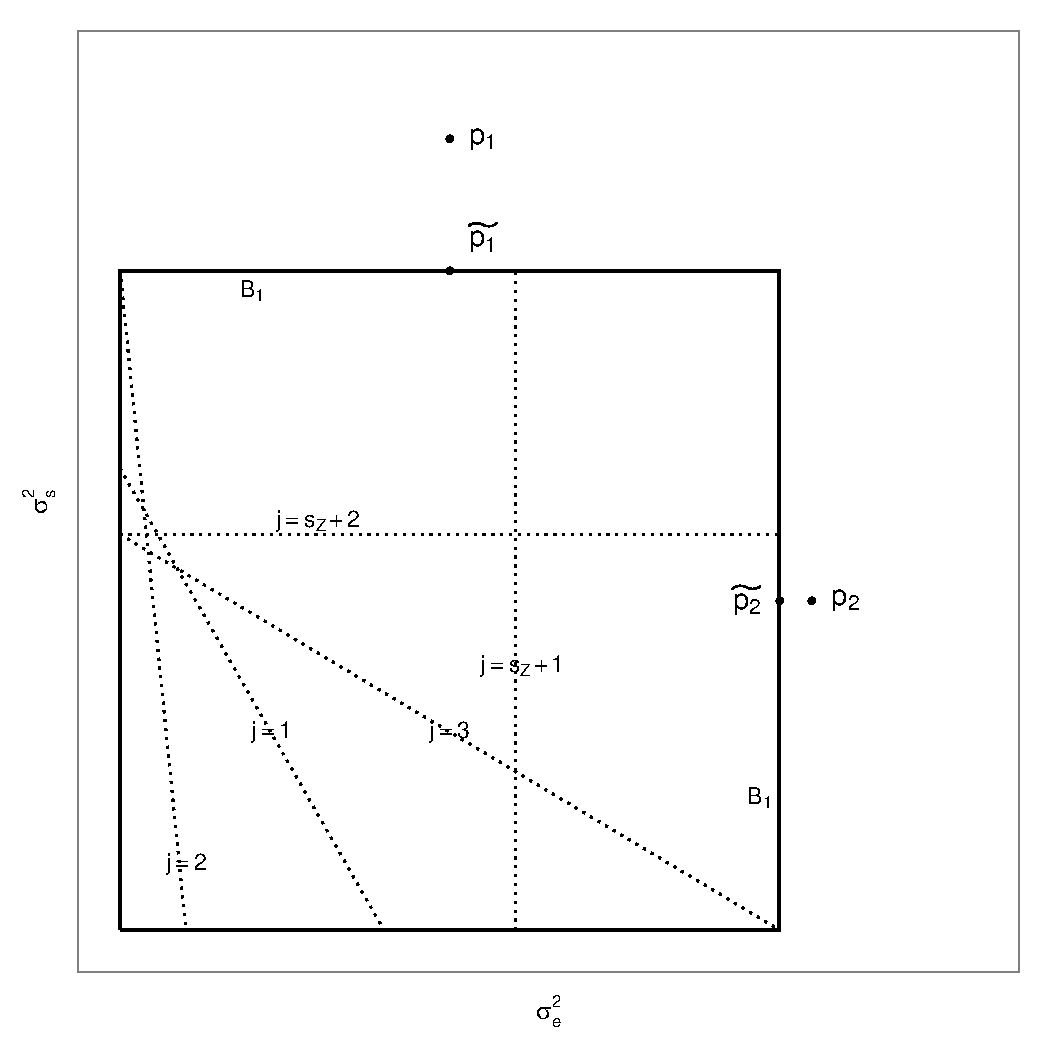
\includegraphics[width=.8\linewidth]{figs/boundingbox.pdf}
	\caption{A rectangular region $B_1$ containing all maxima.}
	\label{fig:bigboundingbox}
  \end{subfigure}
  \begin{subfigure}{.5\textwidth}
	\centering
	\includegraphics[width=.8\linewidth]{figs/smallboundingregion.pdf}
	\caption{A smaller region containing all maxima.}
	\label{fig:smallboundingbox}
  \end{subfigure}
  \caption{all local and global maxima lie in the regions bounded by the solid
                dark line.
               }
  \label{fig:boundingbox}
\end{figure}

By the claim, \mrle\ must lie on or inside $B_1$, so $B_1$ could be passed to an optimizer such as \R's \textsf{optim} or \textsf{nlminb} with potentially better results than using those functions without bounds.  However, even with known bounds, general purpose optimizers may still miss \mrle\ and they emphasize single points of highest local $\logRL$ while possibly ignoring large regions where $\logRL$ is nearly as high \citep[][Section 18.1.1]{hill:1965, hodges:2013}.

We will next find a box $B \supset B_1$ satisfying desideratum \textbf{D1}.  First, though, we pause to note that the region outlined in bold in Figure~(\ref{fig:smallboundingbox}) is a subset of $B_1$ that must also contain \mrle\ by the same reasoning used to prove the previous claim.  But it is not rectangular, hence less convenient than $B_1$, so we don't pursue it further.\\[5pt]

\noindent\textbf{Claim} \emph{For any positive number $M$, there exist positive numbers $\widetilde{\sigma_e^2} > \sigesq{}^M$ and $\widetilde{\sigma_s^2} > \sigssq{}^M$ that determine a box $B \supset B_1$ whose lower-left and upper-right corners are $(0,0)$ and $(\widetilde{\sigma_e^2}, \widetilde{\sigma_s^2})$, respectively, such that
\begin{equation*}
  \sup_{B^c} \logRLss \le \logRL(\sshat) - M.
\end{equation*}}
I.e., \textbf{D1} is satisfied.\\[5pt]
\noindent\textbf{Proof}
Let $p$ be an arbitrary point inside $B_1$, as illustrated in Figure~(\ref{fig:boundingbox2}), and define $L \equiv \logRL(p)$; we use $L$ as a lower bound on $\logRL(\sshat)$.  Let $\widetilde{q_1} = (0,\widetilde{\sigma_s^2})$, the intercept of $B$ and the $\sigssq$ axis; let $\widetilde{q_2} = (\sigma_e^{2*},\widetilde{\sigma_s^2})$; let $\widetilde{q_3} = (\widetilde{\sigma_e^2}, \sigma_s^{2*})$; let $\widetilde{q_4} = (\widetilde{\sigma_e^2},0)$, the intercept of $B$ and the $\sigssq$ axis; and let $\logRL_j$ denote the $j$'th term of \eqref{eq:sum}.  The proof considers in turn four regions $Q_1$, $Q_2$, $Q_3$, and $Q_4$ whose union is $B^c$.  Implicitly, $B$ and $B^c$ are functions of $\widetilde{\sigma_e^2}$ and $\widetilde{\sigma_s^2}$.  The proof shows that $\widetilde{\sigma_e^2}$ and $\widetilde{\sigma_s^2}$ can be chosen large enough so that \textbf{D1} is satisfied on each region.  
\begin{itemize}
\item $Q_1: \sigesq \le \sigesq{}^*$ and $\sigssq \ge \widetilde{\sigssq}$, as illustrated by $q_1$ in
  Figure~\ref{fig:boundingbox2}.  In $Q_1$, by inspection of \eqref{eq:sum} and \eqref{eq:partials},
  \begin{itemize}
  \item for $j \ne s_z+1$,
    \begin{equation*}
      \frac{\partial\logRL_j}{\partial\sigesq} \le 0 \hspace{1cm} \text{and} \hspace{1cm}
      \frac{\partial\logRL_j}{\partial\sigssq} \le 0
    \end{equation*}
    so for any $q \in Q_1$,
    \begin{equation*}
      \logRL_j(q) \le \logRL_j(\widetilde{q_1});
    \end{equation*}
  \item  for $j = s_z+1$,
    \begin{equation*}
      \frac{\partial\logRL_j}{\partial\sigesq} > 0 \hspace{1cm} \text{and} \hspace{1cm}
      \frac{\partial\logRL_j}{\partial\sigssq} = 0
    \end{equation*}
    so for any $q \in Q_1$,
    \begin{equation*}
      \logRL_j(q) \le \logRL_j(\widetilde{q_2}).
    \end{equation*}
  \end{itemize}
  Therefore, 
  \begin{equation}
	\logRL(\sshat) - \logRL(q) \ge L -
	  \sum_{\substack{j=1\\ j \ne s_z+1}}^{s_z+2} \logRL_j(\widetilde{q_1}) - \logRL_{s_z+1}(\widetilde{q_2}).
  \end{equation}
  The r.h.s.~is larger than $M$ if
  \begin{equation}
    \label{eq:q1}
    \begin{split}
      \sum_{\substack{j=1\\ j \ne s_z+1}}^{s_z+2} \logRL_j(\widetilde{q_1})
        &< L - M - \logRL_{s_z+1}(\widetilde{q_2})\\
        &= L - M + \frac{1}{2} \left[ c_{s_z+1}\log\sigma_e^{2*} + \frac{d_{s_z+1}}{\sigma_e^{2*}}\right].
    \end{split}
  \end{equation}
  Examination of (\ref{eq:sum}) shows that for any fixed $\sigesq$, in particular for $\sigesq=0$,
  and for $j \ne s_z+1$,\\ $\lim_{\sigssq \rightarrow \infty} \logRL_j(\sigesq,\sigssq) = -\infty$.
  Thus $\widetilde{\sigma_s^2}$ can be chosen large enough so that the summation on the
  l.h.s.~of \eqref{eq:q1} is less than the r.h.s.~of \eqref{eq:q1}, and  \textbf{D1} is satisfied.
\item $Q_2: \sigesq \ge \sigesq{}^*$ and $\sigssq \ge \widetilde{\sigssq}$, as illustrated by $q_2$ and $q_3$
  in Figure~\ref{fig:boundingbox2}.  In $Q_2$, for all $j$,
  \begin{equation*}
    \frac{\partial\logRL_j}{\partial\sigesq} \le 0 \hspace{1cm} \text{and} \hspace{1cm}
    \frac{\partial\logRL_j}{\partial\sigssq} \le 0
  \end{equation*}
  so for any $q \in Q_2$,
  \begin{equation*}
    \logRL_j(q) \le \logRL_j(\widetilde{q_2}).
  \end{equation*}
  Therefore, $\logRL(\sshat) - \logRL(q) \ge L - \logRL(\widetilde{q_2})$.  The latter expression is greater than
  $M$ iff $\logRL(\widetilde{q_2}) < L-M$.  But (\ref{eq:sum}) shows that for any fixed
  $\sigesq$, $\lim_{\sigssq \rightarrow \infty} \logRLss = -\infty$ and therefore $\widetilde{\sigma_s^2}$
  can be chosen large enough so that \textbf{D1} is satisfied.
\item $Q_3: \sigesq \ge \widetilde{\sigesq}$ and $\sigssq \ge \sigssq{}^*$, as illustrated by $q_3$.  In $Q_3$,
  for all $j$,
  \begin{equation*}
    \frac{\partial\logRL_j}{\partial\sigesq} \le 0 \hspace{1cm} \text{and} \hspace{1cm}
    \frac{\partial\logRL_j}{\partial\sigssq} \le 0
  \end{equation*}
  so for any $q \in Q_3$,
  \begin{equation*}
    \logRL_j(q) \le \logRL_j(\widetilde{q_3}).
  \end{equation*}
  Therefore, $\logRL(\sshat) - \logRL(q) \ge L - \logRL(\widetilde{q_3})$.  The latter expression is greater than
  $M$ iff $\logRL(\widetilde{q_3}) < L-M$.  But for any fixed $\sigssq$,
  $\lim_{\sigesq \rightarrow \infty} \logRLss = -\infty$ and therefore $\widetilde{\sigma_e^2}$
  can be chosen large enough so that \textbf{D1} is satisfied.
\item $Q_4: \sigesq \ge \widetilde{\sigesq}$ and $\sigssq \le \sigssq{}^*$, as illustrated by $q_4$.  In $Q_4$,
  \begin{itemize}
  \item for $j \ne s_z+2$,
    \begin{equation*}
      \frac{\partial\logRL_j}{\partial\sigesq} < 0 \hspace{1cm} \text{and} \hspace{1cm}
      \frac{\partial\logRL_j}{\partial\sigssq} \le 0
    \end{equation*}
    so for any $q \in Q_4$,
    \begin{equation*}
      \logRL_j(q) \le \logRL_j(\widetilde{q_4});
    \end{equation*}
  \item  for $j = s_z+2$,
    \begin{equation*}
      \frac{\partial\logRL_j}{\partial\sigesq} = 0 \hspace{1cm} \text{and} \hspace{1cm}
      \frac{\partial\logRL_j}{\partial\sigssq} \ge 0
    \end{equation*}
    so for any $q \in Q_4$,
    \begin{equation*}
      \logRL_j(q) \le \logRL_j(\widetilde{q_3}).
    \end{equation*}
  \end{itemize}
  Therefore,
  \begin{equation*}
	\logRL(\sshat) - \logRL(q) \ge L - \sum_{j=1}^{s_z+1} \logRL_j(\widetilde{q_4}) - \logRL_{s_z+2}(\widetilde{q_3})
  \end{equation*}
  which is larger than $M$ if
  \begin{equation}
  \label{eq:q4}
    \begin{split}
      \sum_{j=1}^{s_z+1} \logRL_j(\widetilde{q_4})
        &< L - M - \logRL_{s_z+2}(\widetilde{q_3})\\
        &= L - M + \frac{1}{2} \left[ c_{s_z+2}\log\sigma_s^{2*} + \frac{d_{s_z+2}}{\sigma_s^{2*}}\right].
    \end{split}
  \end{equation}
  For any fixed $\sigssq$, in particular for $\sigssq=0$, and for $j \ne s_z+2$,\\ $\lim_{\sigesq \rightarrow \infty}
  \logRL_j(\sigesq,\sigssq) = -\infty$.  Thus $\widetilde{\sigma_e^2}$ can be chosen large enough so that the
  summation on the l.h.s.~of \eqref{eq:q4} is less than the r.h.s.~of \eqref{eq:q4}, and  \textbf{D1} is satisfied.\end{itemize}  
\textbf{QED}\\

\begin{figure}[h]
	\centering
	\includegraphics[width=.5\linewidth]{figs/boundingbox2.pdf}
	\caption{Box $B$ satisfies (\ref{eq:boundingbox})}
	\label{fig:boundingbox2}
\end{figure}

\subsection{Lines Determine Bounds within Boxes}
\label{sec:boundsinboxes}
\begin{figure}
	\centering
	\includegraphics[width=.5\linewidth]{figs/boxb.pdf}
	\caption{For a box $b$,  the minimum and
	maximum within $b$ of $\logRL_j$
	occur at either the lower left corner, the upper right  corner, or
	on the line.
}	\label{fig:boxb}
\end{figure}
Next we consider the relationship between the $\logRL_j$'s and boxes as depicted in Figure~\ref{fig:boxb}, which shows a small box $b$ and three lines.  For lines such as $j=2$ that lie below or to the left of $b$, the partial derivatives (\ref{eq:drlds}, \ref{eq:drlde}) are nonpositive, so the maximum and minimum of $\logRL_j$ within $b$ are attained at the lower left and upper right corners respectively.  The situation is reversed for lines like $j=3$ that lie above or to the right of $b$: the partial derivatives are nonnegative so the maximum and minimum are attained at the upper right and lower left corners respectively.  For lines like $j=1$ that pass through $b$, the minimum is attained at either the upper right or lower left corner while the maximum is attained on the line.

For any box $b$ let $L^b_j = \inf_{p\in b} \logRL_j(p)$ and $U^b_j = \sup_{p\in b} \logRL_j(p)$.  We have just shown that $L^b_j$ and $U^b_j$ are easily computable by evaluating $\logRL_j$ at either two points (two corners for lines like $j=2,3$) or three points (two corners and one on the line for lines like $j=1$).
Armed with the $L^b_j$'s and $U^b_j$'s we can compute bounds on $\logRLss$ within $b$:
\begin{equation}
\label{eq:bounds}
	L^b \equiv \sum_{j=1}^{s_z+2} L^b \le \inf_{(\sigssq,\sigesq)\in b} \logRLss \le
	\sup_{(\sigssq,\sigesq)\in b} \logRLss \le \sum_{j=1}^{s_z+2} U^b_j \equiv U^b.
\end{equation}
Because $\logRL$ is continuous, $U^b - L^b \rightarrow 0$ as $b$ shrinks in both directions, thus satisfying desideratum \textbf{D2}.

\section{An Algorithm}
\label{sec:algorithm}
Section~\ref{sec:boundingbox} shows how to determine a box $B_1$ containing all local maxima of $\logRLss$ and   that we can find a bigger box $B\supseteq B_1$ satisfying \textbf{D1}.  We are about to present an algorithm that uses Section~\ref{sec:boundsinboxes} to show that any bounded box $B^0$ can be partitioned into finitely many smaller boxes $B^0_1, \dots B^0_p$  such that, for each $B^0_i$ in the partition, we know for pre-specified constants $M, \epsilon >0$, either
\begin{enumerate*}[label=(\alph*)]
\item $\sup_{B^0_i} \logRL < \sup_{B^0} \logRL -M$ or
\item $\sup_{B^0_i} \logRL - \inf_{B^0_i} \logRL < \epsilon$.
\end{enumerate*}
If $B^0$ satisfies \textbf{D1} and $B^0\supseteq B_1$ then we have accomplished our goal of dividing the plane into one region where we know $\logRL$ to be low and another where we know $\logRL$ to within $\epsilon$.  One strategy would be to find $B$ as outlined in Section~\ref{sec:boundingbox} and set $B^0 \equiv B$.  However, we have found that $B_1$ satisfies \textbf{D1} in all the examples we have tried and we therefore follow a different strategy.  We set $B^0 \equiv B_1$ and run the following algorithm, during which we learn whether $B_1$ satisfies \textbf{D1}.  If it does, we're done.  If it doesn't, then we would expand $B_1$ by a factor of 2 in both dimensions; set $B^0$ to be the expanded box; rerun the algorithm; and continue to expand and rerun until we find a $B^0$ that does satisfy \textbf{D1}.  Section~\ref{sec:boundingbox} shows that such a bounded $B^0$ exists, and thus we are sure to find it in finite time.

Algorithm~\ref{alg:findf} sketches the basic procedure; details are in an appendix.  Before giving examples, we mention some considerations in setting the tuning constants $M$ and $\epsilon$, which have to do with the interpretation of likelihood ratios.  We imagine a reference experiment in which a coin is chosen, either fair or two-headed, and tossed.  If the coin is tossed twice and lands Heads both times, it produces a likelihood ratio of 4 in favor of the two-headed coin.  That's only weak evidence, so we don't see the need to resolve likelihood functions much beyond a factor of four, or loglikelihood functions much beyond a factor of $\log(4) \approx 1.4$.  In practice, we use $\epsilon = 1$ as a convenient default.  If the coin were tossed 10 times and yielded 10 Heads, the likelihood ratio would be $2^{10} = 1024$.  That's strong evidence, so we don't see the need to resolve $\logRL$ where it is less than .001 times its maximum.  $\log(1000) \approx 7$, so we use $M = 7$ as a convenient default.

\begin{algorithm}[H]
  \caption{Learn areas in $B$ where log $f$ is high to within $\epsilon$
    \label{alg:findf}}
  \begin{algorithmic}[1]
    \Function{findf}{$B, \epsilon, M$}
      \Let{$active$}{list containing only $B$}
      \Let{$inactive$}{empty list}
      \Let{$L$}{$-\infty$}
      \While{length of $active > 0$}
        \For{each element $b$ in $active$}
          \Let{$L^b, U^b$}{get bounds on log $f$ in $b$ \Comment{see section \ref{sec:boundsinboxes}}}
        \EndFor
          \Let{tmp}{max($L^b$)}
         \Let{$L$}{max($L$, tmp)}
        \For{each element $b$ in $active$}
          \If{$U^b - L^b < \epsilon \enspace \textrm{or} \enspace U^b < L - M$}
            \State move $b$ from $active$ to $inactive$
          \Else
            \Let{$b_1, b_2, b_3, b_4$}{split $b$ into 4 smaller boxes}
            \State remove $b$ from $active$
            \State add $b_1, b_2, b_3, b_4$ to $active$
          \EndIf
        \EndFor
      \EndWhile
      \State \Return $inactive$ 
    \EndFunction
  \end{algorithmic}
\end{algorithm}


\section{Examples}
\label{sec:examp}
Section~\ref{sec:examp}'s examples use $\epsilon = 1$ and $M = 7$.
Computations were performed on an iMac that was new in 2011, having a 2.7 GHz Intel Core i5 processor and 4GB of memory.
\subsection{HMO premiums}
\subsubsection{Introduction to the Data}
Our first example is a traditional linear mixed model previously analyzed in \citet{hodges:98},  \cite{wakefield:1998}, \cite{hodges:2013}, and \cite{henn&hodges:2014}. \cite{wakefield:1998} reported a bimodal log posterior density for $(\sigesq,\sigssq)$.  Quoting from \cite{henn&hodges:2014},
\begin{quote}
\itshape
\dots the HMO data set describes 341 HMOs [Health Maintenance Organizations] located in 45 states or similar political jurisdictions.  Each jurisdiction had between 1 and 31 plans with a median of 5 plans.  The data set originally was analysed to assess the cost of moving military retirees and dependents from a Department of Defense health plan to plans serving the US civil service.  \dots.  Specifically, the model is
\begin{equation*}
\begin{split}
	y_{ij} &= \alpha_i + \epsilon_{ij}\\
	\alpha_i &= \varrho_0 + \varrho_1x_{1i} + \varrho_2x_{2i} + \zeta_i,
\end{split}
\end{equation*}
where the fixed effects in $\alpha_i$ include an intercept, jurisdiction-average hospital expenses per admission ($x_{1i}$) and an indicator for plans in New England states ($x_{2i}$).

\upshape
\end{quote}
I.e., $X$ is a $341 \times 3$ matrix with columns for the intercept and two fixed effects and $Z$ is a $341 \times 45$ matrix whose columns are indicators of the 45 jurisdictions.  The data are available at \url{http://www.biostat.umn.edu/~hodges/RPLMBook/Datasets/09_HMO_premiums/Ex9.html}.  Because the span of $Z$'s columns contains the span of $X$'s, $s_z = 42$.  

\subsubsection{A log RL Analysis}
For a $\logRLssorig$ analysis there are 43 lines, as shown in Figure~\ref{fig:hmolines}.
Running the algorithm on the box $B_1$ determined by the lines' maximum intercepts on the $\sigesq$ and $\sigssq$ axes results in the the output displayed in Table~\ref{table:hmo_HH11_run}, which shows the state of the algorithm after iterations 1 through 15: the numbers of active and inactive boxes and the current value of the lower bound $L$ on $\max\log f$. The run finished in less than 10 seconds.  We see that boxes are steadily transferred from the active to the inactive list and that $L$ increases monotonically.  After 15 iterations there is a total of 9490 boxes, which are displayed in Figure~\ref{fig:hmo1}.

\begin{table}[h]
\centering
\begin{tabular}{|c|c|c|c|}
\hline
Iteration & $n$ active boxes & $n$ inactive boxes & $L$\\
1 & 4 & 0 & $-\infty$\\
2 & 16 & 0 & -1618.84\\
3 & 40 & 6 & -1509.24\\
4 & 72 & 28 & -1408.12\\
5 & 144 & 64 & -1325.99\\
6 & 68 & 191 & -1265.01\\
7 & 116 & 230 & -1256.35\\
8 & 144 & 310 & -1243.51\\
9 & 340 & 369 & -1240.05\\
10 & 920 & 479 & -1237.87\\
11 & 2540 & 764 & -1236.79\\
12 & 4380 & 2209 & -1236.20\\
13 & 3524 & 5708 & -1235.90\\
14 & 344 & 9146 & -1235.90\\
15 & 0 & 9490 & -1235.90\\
\hline
\end{tabular}
\caption{The state of the algorithm after each of 15 iterations for the HMO data.}
\label{table:hmo_HH11_run}
\end{table}

\begin{figure}
	\centering
	\includegraphics[width=.45\linewidth]{figs/hmo_HH11_lines.pdf}
	\caption{The 43 lines, $j=1, 2, \dots, 43$, for the $\logRLorig$ analysis of the HMO data.
	              The line for $j = s_z+1 = 43$ is dashed.}
	\label{fig:hmolines}
\end{figure}

\begin{figure}
  \begin{subfigure}{.5\textwidth}
	\centering
	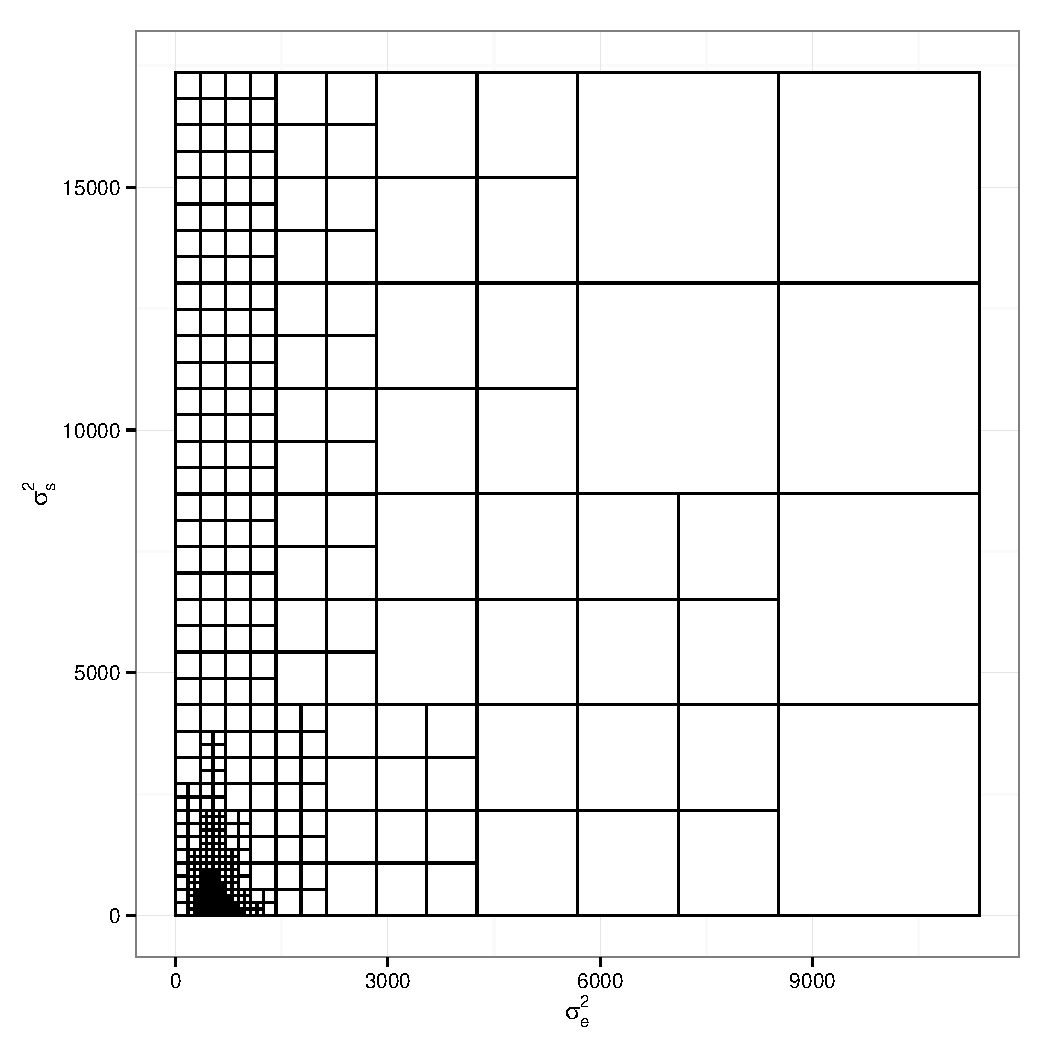
\includegraphics[width=.8\linewidth]{figs/hmo_HH11_boxes.pdf}
	\caption{Locations of the boxes.}
	\label{fig:hmoboxes}
  \end{subfigure}
  \begin{subfigure}{.5\textwidth}
	\centering
	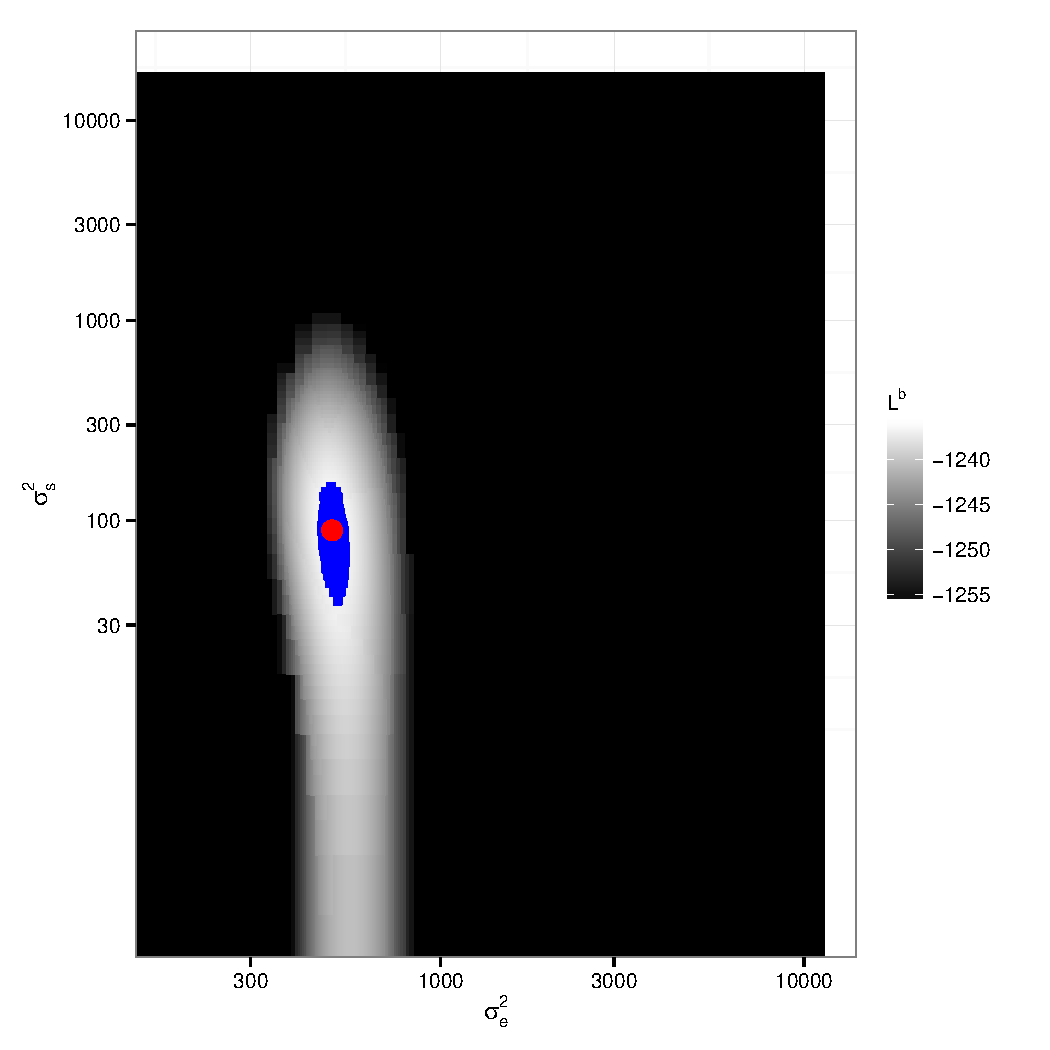
\includegraphics[width=.8\linewidth]{figs/hmo_HH11_rll.pdf}
	\caption{Grayscale shows $L^b$ in each box.  Red dot shows $b^* \equiv\argmax L^b$.
	Boxes outlined in blue have $U^b \ge L^{b^*}$.  Axes are logarithmic.}
	\label{fig:hmorll}
  \end{subfigure}
  \caption{The 9490 boxes produced in the
	$\logRLorig$ analysis of the HMO data. $\maxit=\infty; \epsilon=1;
	\delta_e= \delta_s= 0; \text{and\ } M=7$.}
  \label{fig:hmo1}
\end{figure}

Figure~\ref{fig:hmoboxes} shows the outlines of the 9490 boxes.  The algorithm did not need to divide the boxes with large $\sigesq$ or $\sigssq$ as finely as those with small $\sigesq$ and $\sigssq$ because they more readily satisfy either $U^b < L-M$ or $U^b - L^b < \epsilon$, so become inactive.  Figure~\ref{fig:hmorll} shows the same boxes on a logarithmic scale, shaded by $L^b$ in each box.  The red dot is the lower left corner of the box that maximizes $L^b$.  Boxes with $U^b \ge L \equiv \max L^b$ are outlined in blue; $(\sshat)$ must lie within the blue region.  
For comparison, the standard REML analysis using \R's \textcompute{lme} function yields $\sshat \approx (495, 99)$ with 95\% confidence intervals of $(421, 582)$ and $(39, 248)$.

Figure~\ref{fig:hmorll} depicts the same $\logRLorig$ as \cite{henn&hodges:2014}'s Figures~2a (MCMC draws) and~2b ($\logRLorig$ contours), but their Figure~2a was produced by MCMC whereas our Figure~\ref{fig:hmorll} was produced by direct calculation.  Their Figure~2a shows that the MCMC sampler did not sample any values of $\sigssq$ less than about 10, whereas our Figure~\ref{fig:hmorll} and their Figure~2b show a region of high $\logRLorig$ extending down to $\sigssq=0$.  In fact, $\logRLorig(500,0) \approx -1241.5$, only about 6 log units below $\logRLorig(\sshat) \approx -1235.7$.  Further, about their Figure~2a, Henn and Hodges say, ``No change in contour shape indicative of a local maximum could be found in the \dots region of $(500, 600) \times (10^{-3}, 1)$, regardless of contour resolution."  I.e., they cannot be sure there are no undiscovered points with large $\logRLorig$.  In contrast, our algorithm guarantees there are no undiscovered points where $\logRLorig$ is more than $\epsilon$ above $L$.

\subsubsection{A Bayesian Analysis}
 \cite{hodges:98}, \cite{wakefield:1998}, \cite{hodges:2013}, and \cite{henn&hodges:2014} report  Bayesian analyses of the HMO data.  Here we reproduce the analysis from \cite{hodges:98} which used inverse Gamma priors for $(\sigesq,\sigssq)$ with $\alpha_e = 1$; $\beta_e = 0$; $\alpha_s = 1.1$; and $\beta_s =0.1$.  (We don't defend the prior; we use it so we can compare to Hodges.)

For a Bayesian analysis there are 44 lines, as shown in Figure~\ref{fig:hmoBayeslines}.  Figure~\ref{fig:hmoBayeslines} differs from Figure~\ref{fig:hmolines} in that it includes a horizontal line for $j = s_z+2$ and the position of the vertical line for $j = s_z+1$ is slightly shifted.
\begin{figure}
	\centering
	\includegraphics[width=.45\linewidth]{figs/hmolines_HH11_Bayes.pdf}
	\caption{The 44 lines, $j=1, 2, \dots, 44$, for the Bayesian analysis of the HMO data.
	              Lines 43 and 44 are dashed.}
	\label{fig:hmoBayeslines}
\end{figure}
Because the $\logRLorig$ analysis in Figure~\ref{fig:hmorll} shows low values for $\sigesq, \sigssq > 1000$, we run the Bayesian analysis on the box $B^0 = (0,1000) \times (0,1000)$.
The algorithm finished in 22 iterations and took a little under 3 hours.  Table~\ref{table:hmo_HH11Bayes} shows the output and Figure~\ref{fig:hmoBayes} shows the boxes.
\begin{table}[H]
\centering
\begin{tabular}{|c|c|c|c|}
\hline
Iteration & $n$ active boxes & $n$ inactive boxes & $L$\\
1 & 4 & 0 & $-\infty$\\
2 & 16 & 0 & -1313.42\\
3 & 52 & 3 & -1285.05\\
4 & 132 & 22 & -1270.76\\
5 & 264 & 88 & -1263.98\\
6 & 628 & 195 & -1260.47\\
7 & 1780 & 378 & -1258.71\\
8 & 4188 & 1111 & -1257.70\\
9 & 5676 & 3880 & -1256.88\\
10 & 5136 & 8272 & -1255.56\\
11 & 5528 & 12026 & -1254.20\\
12 & 8236 & 15495 & -1252.84\\
13 & 12488 & 20609 & -1251.50\\
14 & 23852 & 27134 & -1250.26\\
15 & 22740 & 45301 & -1249.22\\
16 & 43228 & 57234 & -1248.77\\
17 & 160208 & 60410 & -1248.77\\
18 & 331900 & 137643 & -1248.77\\
19 & 575196 & 325744 & -1248.77\\
20 & 942860 & 665225 & -1248.77\\
21 & 722412 & 1427482 & -1248.77\\
22 & 0 & 2149894 & -1248.77\\
\hline
\end{tabular}
\caption{The state of the algorithm after each of 22 iterations for the Bayesian analysis of the HMO data.}
\label{table:hmo_HH11Bayes}
\end{table}
The Bayesian analysis in Figure~\ref{fig:hmoBayes} can be compared to the $\logRLorig$ analysis in Figure~\ref{fig:hmo1}.  The peak of the log posterior is near $(600, .05)$, very far from the peak of the $\logRLorig$ around $(500,100)$.  The posterior peak is due to the $\IG(1.1,0.1)$ prior for $\sigssq$, which has a mean of 1, an infinite variance, and a peak at 0.048.  The region near $(500,100)$, though having a lower posterior density, is part of a nearly flat plateau covering a large area.  The MCMC draws depicted in \cite{henn&hodges:2014} Figure~2c show that the plateau has significant posterior mass.

\begin{figure}
  \begin{subfigure}{.5\textwidth}
	\centering
	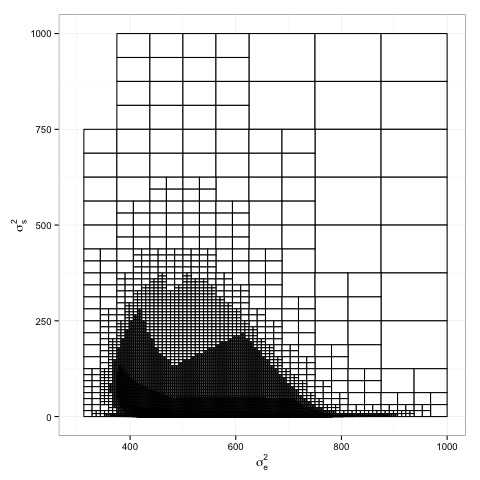
\includegraphics[width=.8\linewidth]{figs/hmo_HH11Bayes_boxes.jpg}
	\caption{Locations of the boxes.}
	\label{fig:hmoBayesboxes}
  \end{subfigure}
  \begin{subfigure}{.5\textwidth}
	\centering
	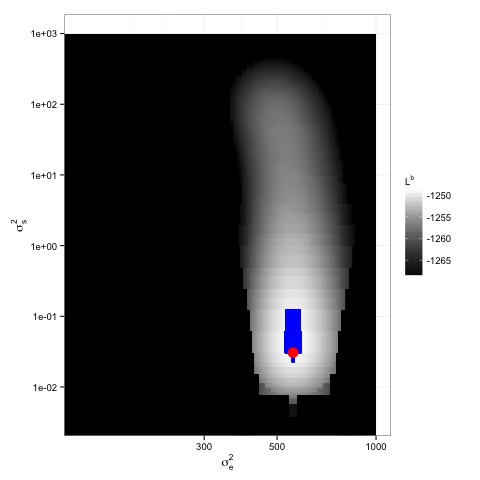
\includegraphics[width=.8\linewidth]{figs/hmo_HH11Bayes_rll.jpg}
	\caption{Grayscale shows $L^b$ in each box.  Red dot shows $b^* \equiv\argmax L^b$.
	Boxes outlined in blue have $U^b \ge L^{b^*}$.  Axes are logarithmic.}
	\label{fig:hmoBayesrll}
  \end{subfigure}
  \caption{The 2,149,894 boxes in the Bayesian analysis of the HMO data.}
  \label{fig:hmoBayes}
\end{figure}

\subsection{Global Mean Surface Temperature}
We reanalyze a data set in \cite{hodges:2013}, global mean surface temperatures (GMST) from 1881 through 2005, depicted in Figure~\ref{fig:gmst-scatter}.  
\begin{figure}
	\centering
	\includegraphics[width=.5\linewidth]{figs/gmst-scatter.pdf}
	\caption{Global mean surface temperature annually from 1881.
		The $y$-axis shows deviations from the overall mean in units of
		.01 degrees C.}
	\label{fig:gmst-scatter}
\end{figure}
As shown in \cite{ruppert_etal:2003}, many splines can be written as linear mixed models.  \cite{hodges:2013} fit a piecewise quadratic spline to the GMST data, though a piecewise cubic spline would look similar.  Both splines can be formulated as linear mixed models.  We follow his lead in fitting a quadratic spline with knots at 1880, 1884, 1888, \dots, 2004.  $X$ has three columns: $\textcompute{1}, \textcompute{year}, \textcompute{year}^2$.  $Z$ is $125 \times 30$: one row for each year; one column for each knot.
%\begin{equation*}
%Z =	\begin{bmatrix}
%		0 & 0 & \dots & 0\\
%		0 & 0 & \dots & 0\\
%		0 & 0 & \dots & 0\\
%		0 & 0 & \dots & 0\\
%		1 & 0 & \dots & 0\\
%		4 & 0 & \dots & 0\\
%		9 & 0 & \dots & 0\\
%		16 & 0 & \dots & 0\\
%		25 & 1 & \dots & 0\\
%		\vdots & \vdots & \vdots & \vdots\\
%		13924 & 12996 & \dots & 4\\
%		14161 & 13225 & \dots & 9\\
%		14400 & 13456 & \dots & 16\\
%		14641 & 13689 & \dots & 25\\
%	\end{bmatrix}; \hspace{.5cm} \Sigma_e = \mathbf{1}_{125}; \hspace{.5cm}
%		\Sigma_s = \mathbf{1}_{30}
%\end{equation*}
Because we fit a quadratic spline, the entries in $Z$ are squares.  $\Sigma_e$ and $\Sigma_s$ are identity matrices of the appropriate dimension; see \cite{hodges:2013} for details.  Following Hodges, we center and scale the \textcompute{year} column of X, then compute the $\textcompute{year}^2$ column of $X$ and all the columns of Z from the transformed \textcompute{year}, so Z becomes
\begin{equation*}
Z =	\begin{bmatrix} 
		0 & 0 & \dots & 0\\
		\vdots & \vdots & \vdots & \vdots\\
		10.97143 & 10.2521 & \dots & 0.01219048\\
		11.15505 & 10.42971 & \dots & 0.01904762\\
	\end{bmatrix}
\end{equation*}
Centering and scaling changes only the scale on which $\sigssq$ is measured; we do it to more easily compare our result to Hodges'.

The column space of $Z$ shares no dimensions with the column space of $X$ so $s_z=30$ and, for our $\logRLorig$ analysis, there are 31 lines in all, as shown in Figure~\ref{fig:gmst-lines}.
\begin{figure}
	\centering
	\includegraphics[width=.5\linewidth]{figs/gmst-lines.pdf}
	\caption{The 31 lines for the $\logRLorig$ analysis of
	              global mean surface temperatures.}
	\label{fig:gmst-lines}
\end{figure}
As usual, we use $B^0 = B_1$, the box determined by the largest intercepts of the 31 lines on the $\sigesq$ and $\sigssq$ axes.
%and the control constants 
%\begin{equation*}
%	\maxit=\infty; \hspace{1cm} \epsilon=1; \hspace{1cm}
%	\delta_e= \delta_s=0; \hspace{1cm} M=7.
%\end{equation*}
After 25 iterations and about 35 minutes of computing time, all boxes became inactive.  Output is in Table~\ref{table:gmst_output}; boxes are displayed in Figure~\ref{fig:gmst1}.
\begin{table}%[H]
\centering
\begin{tabular}{|c|c|c|c|}
\hline
Iteration & $n$ active boxes & $n$ inactive boxes & $L$\\
1 & 4 & 0 & $-\infty$\\
2 & 16 & 0 & -560.82\\
3 & 48 & 4 & -519.98\\
4 & 84 & 31 & -480.58\\
5 & 152 & 77 & -446.67\\
6 & 184 & 183 & -419.47\\
7 & 176 & 323 & -406.31\\
8 & 164 & 458 & -395.36\\
9 & 284 & 551 & -390.24\\
10 & 496 & 711 & -385.84\\
11 & 984 & 961 & -382.45\\
12 & 1792 & 1497 & -379.65\\
13 & 2880 & 2569 & -377.36\\
14 & 4668 & 4282 & -375.37\\
15 & 7312 & 7122 & -373.66\\
16 & 10336 & 11850 & -372.29\\
17 & 10108 & 19659 & -371.21\\
18 & 18596 & 25118 & -370.82\\
19 & 62488 & 28092 & -370.82\\
20 & 124240 & 59520 & -370.70\\
21 & 287596 & 111861 & -370.70\\
22 & 494292 & 275884 & -370.70\\
23 & 646808 & 608474 & -370.70\\
24 & 291944 & 1182296 & -370.70\\
25 & 0 & 1474240 & -370.70\\
\hline
\end{tabular}
\caption{The state of the algorithm after each of 25 iterations for the GMST data.}
\label{table:gmst_output}
\end{table}


\begin{figure}
  \begin{subfigure}{.5\textwidth}
    \centering
    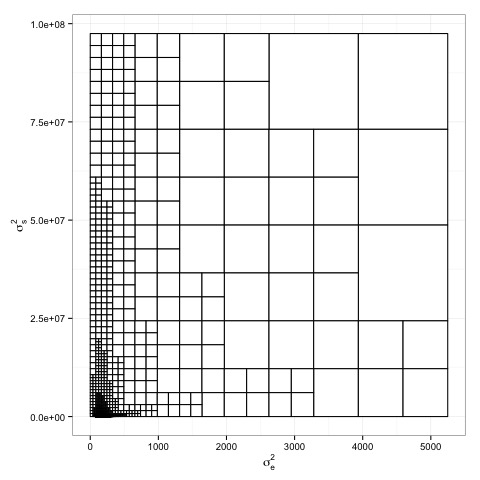
\includegraphics[width=.8\linewidth]{figs/gmst-boxes1.jpg}
    \caption{Locations of boxes}
    \label{fig:gmst-boxes1}
  \end{subfigure}
  \begin{subfigure}{.5\textwidth}
    \centering
    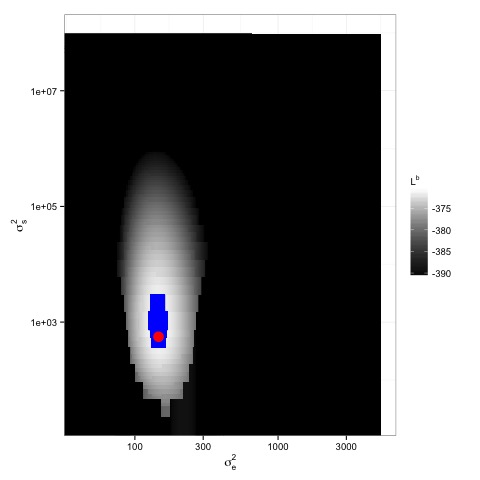
\includegraphics[width=.8\linewidth]{figs/gmst-rll1.jpg}
    \caption{Grayscale shows $L^b$ in each box.
                  Red dot shows $b^* \equiv\argmax L^b$.
	          Boxes outlined in blue have $U^b \ge L^{b^*}$.
	          Axes are logarithmic.}
    \label{fig:gmstrll1}
  \end{subfigure}
  \caption{The 1,474,240 boxes from the analysis of global mean surface temperature.}
\label{fig:gmst1}
\end{figure}
The figure shows that the algorithm needed to divide boxes near the axes more finely than boxes away from the axes and that high $\logRLorig$ is found near $(200, 1000)$.  The figure agrees with Figure~15.3 in \cite{hodges:2013}.

\section{Discussion}
This paper explains and illustrates an algorithm that facilitates computation for linear mixed models with two variances. The algorithm finds all regions where either the restricted likelihood function or the joint posterior density of the variances is high and can evaluate the function there to arbitrary accuracy.  A natural question to ask is \emph{What about linear mixed models with more than two variances?}  A partial answer is given by \cite{hodges:2013} who shows that some models with more than two variances can be re-expressed similarly to \eqref{eq:reexpress} but others can't.  More complex models that can be re-expressed this way include, but are probably not limited to, models displaying general balance that are also orthogonal designs \citep[all balanced ANOVAs plus other models;][]{houtman_speed:1983}, models that are separable in a specific sense \citep[Section 17.1.5]{hodges:2013}, and miscellaneous other models \citep[Section 17.1.5]{hodges:2013}, e.g., a spatial model including random effects for heterogeneity and spatial clustering (an improper conditional autoregressive effect). We have not explored whether the re-expressible models can be analyzed by our algorithm; that's one direction for future work.  

Another is to see whether the algorithm can be used to advantage even in non-re-expressible models.  If a model has, say, three variances and is now analyzed by, say, MCMC, we can create an MCMC chain that alternates between draws of $(\sigesq,\sigssq)$ and draws of the other variance.  With the aid of our algorithm we may be able to draw more accurately from $[\sigesq,\sigssq\g \sigma^2_\text{other}]$.  More generally, the conditional distribution of $(\sigesq,\sigssq)$ given other parameters can now be analyzed more accurately than in the past.  We have yet to explore how to exploit that accuracy.  A third direction is the posterior $\pi(\sigesq,\sigssq\g y)$.  We can identify a region $B^c$ where the posterior density is low relative to its maximum and it would be of at least mild interest to find an upper bound for the posterior mass of $B^c$.

As written, our algorithm moves a box $b$ to the inactive list if
\begin{enumerate*}[label=(\alph*)]
\item $U^b < L-M$ or
\item $U^b - L^b < \epsilon$.
% \item either the vertical or horizontal extent of $b$ is sufficiently small.
\end{enumerate*}
But one could construct more elaborate rules.  One appealing example is to apply criterion (a) if $U^b \le L-\epsilon_2$ and apply criterion (b) if $U^b > L-\epsilon_2$.  Other rules are possible, too.  We don't elaborate here in order to concentrate on the main ideas.

More generally, our algorithm differs from typical optimization algorithms in that it has a different goal: learning $\logRL$ to specified accuracy wherever $\logRL$ is high.  The algorithm works by exploiting a re-expression of $\logRL$ as a sum of simpler, easily analyzed functions.  But there may be many other statistically interesting functions that can be so re-expressed.  For example, many likelihood functions are products of terms from conditionally independent parts of the data.  Posterior densities have the same terms, plus a term from the prior.  We have not yet explored whether our algorithm, and more generally the idea of learning $\logRL$ to specified accuracy, is useful outside the family of linear mixed models; that's another direction for future work.

In this paper we have taken the point of view that it is important to find all regions where $\log f$ is large without necessarily identifying all local maxima or even the global maximum, even though that point of view is at odds with common statistical estimators that maximize the likelihood, the restricted likelihood, or the posterior density.  If two local maxima are close in height it hardly matters which is slightly higher than the other.  And, as we said earlier, if there is a high plateau it hardly matters whether there are little bumps on that plateau.

\appendix
\section{Appendix: Derivation of $\{a_j\}$ and $\{\hat v_j\}$ in \eqref{eq:reexpress}, \eqref{eq:logpost}, and \eqref{eq:sum}}
Our derivation follows \cite{hodges:2013},
which contains more details.  There are three steps.
\begin{enumerate}
  \item \textbf{Make the covariance matrices proportional to the identity.}  If $\Sigma_e$ is not the identity matrix,
    transform the data to $\Sigma_e^{-.5}y$.  The transformed data, which we shall still call $y$, has covariance
    proportional to the identity.  Similarly, if $\Sigma_s$ is not the identity matrix, re-parameterize the random
    effects to $\Sigma_s^{-.5}u$.  The re-parameterized random effects, which we shall still call $u$, have
    covariance proportional to the identity.
  \item \textbf{If the column spaces of $X$ and $Z$ have a non-trivial intersection, transform them.}
    Let $s_X=\text{rank}(X)$  and $s_Z=\text{rank}(X|Z) - s_X$.  Let $\Gamma_X$ be an $n \times s_X$ matrix whose
    columns are an orthonormal basis for the column space of $X$.  Let $\Gamma_Z$ be an $n \times s_Z$ matrix
    such that the columns of $\left[\Gamma_X | \Gamma_Z \right]$ are an orthonormal basis for the column space
    of $\left[X|Z\right]$.  Let $\Gamma_c$ be an $n \times (n-s_X-s_Z)$ matrix such that the columns of
    $\left[\Gamma_X | \Gamma_Z | \Gamma_c\right]$ are an orthonormal basis for $\mathbb{R}^n$.  Define the matrix
    \begin{equation*}
      M = \begin{bmatrix}
               M_{XX} & M_{XZ}\\
               0 & M_{ZZ}
             \end{bmatrix}
    \end{equation*}
    by $[X|Z] = [\Gamma_X|\Gamma_Z]M$ where $M_{XX}$ is $s_X \times p$ and $M_{XZ}$ is $s_Z \times q$.
    $\Gamma_X$ and $\Gamma_Z$ are transformed versions of $X$ and $Z$ that have non-overlapping
    column spaces.
  \item \textbf{Re-parameterize and diagonalize.}  Let $M_{ZZ}$ have the singular value decomposition
    $PA^{.5}L^t$.  Now the linear mixed model \eqref{eq:lmm} can be written as
    \begin{equation*}
      \begin{split}
        y &= \begin{bmatrix} X | Z \end{bmatrix} \begin{bmatrix} \beta \\ u \end{bmatrix} + \epsilon\\
        &= \begin{bmatrix} \Gamma_X | \Gamma_Z \end{bmatrix} M \begin{bmatrix} \beta \\ u \end{bmatrix} + \epsilon\\
        &= \begin{bmatrix} \Gamma_X | \Gamma_Z P \end{bmatrix} \begin{bmatrix} \beta^* \\ v \end{bmatrix} + \epsilon
      \end{split}
    \end{equation*}
    where $\beta^* = M_{XX}\beta + M_{XZ}u$ and $v = A^{.5}L^t u$.  $\beta^*$ contains the re-parametrized
    fixed effects while $v$ contains the re-parametrized random effects.  The corresponding design matrices
    $\Gamma_X$ and $\Gamma_Z P$ are orthogonal to each other.
\end{enumerate}
Finally, the $\{a_j\}$ in \eqref{eq:reexpress} are the diagonal elements of $A$, all of which are strictly positive, and the $\{\hat v_j\}$ in \eqref{eq:reexpress} are given by $\hat v = (\hat v_1, \dots, \hat v_{s_Z})^t = P^t \Gamma_Z^t y$.

\section{Appendix: Details of the algorithm}
With \textbf{D1} and \textbf{D2} the \textcompute{R} function \textcompute{findf}, sketched below, will evaluate, within a box $B^0$, $\logRL$ to arbitrary accuracy everywhere $\logRL$ is large by performing the following tasks:
\begin{enumerate*}[label=(\alph*)]
\item accept as input $\{a_j, b_j, c_j, d_j\}, B^0$ and some tuning constants;
\item create a list of active boxes, initially consisting of just $B^0$;
\item create a list of inactive boxes, initially empty; and
\item for each active box $B_j$, find $(L^{B_j}, U^{B_j})$ and determine whether $B_j$ needs to be subdivided.
\end{enumerate*}
 These notes explain some parts of the function in more detail.
\begin{enumerate}
\item A dataframe \textcompute{lines} is an input to \textcompute{findf}.  \textcompute{lines} contains the
  $\{a_j, b_j, c_j, d_j \}$ from Section~\ref{subsec:lines}.
  Details for computing them from $y$, $X$, $Z$, $\Sigma_e$, and $\Sigma_s$ are in the Appendix.
\item \textcompute{startbox}, or $B^0$, is an input to \textcompute{findf}.  As explained at the beginning of
  Section~\ref{sec:algorithm}, \textcompute{startbox} could be $B_1$, $B$, or any other box the user chooses.
\item Constants \maxit, $M$, $\epsilon$, $\delta_e$, and $\delta_s$ are inputs to \textcompute{findf}.
	\begin{enumerate}[label=(\alph*)]
	\item Though not mentioned in the main text, \maxit\ is the maximum number (could be $\infty$) of iterations of
		\textcompute{findf}'s loop.
	\item We will not further analyze regions of the plane where
		$\logRLss < \logRL(\sshat) - M$.  ($M$ could be $\infty$.)
	\item We will evaluate $\logRL$ to within an accuracy of $\epsilon$ (could be 0) inside $B^0$
	         unless evaluation is stopped by one of the other criteria.
	\item Though not mentioned in the main text, the algorithm can be told not
		to distinguish values of $\sigesq$ separated by less
		than $\delta_e$ (could be 0) nor values of $\sigssq$ separated by
		less than $\delta_s$ (could be 0).  Separation may be specified
		in either absolute or relative terms. (I.e.\ we look at either the difference
		in $\sigesq$ or $\log\sigesq$ (or $\sigssq$ or $\log\sigssq$) from one
		side of the box to the other.)
	\end{enumerate}
  Setting $\maxit = \infty$ and $\delta_e = \delta_s = 0$, as we have done in the examples, implies
  that $B^0$ will be partitioned so that either
  $\logRL < \logRL(\sshat) - M$ or $\logRL$ is known to within $\epsilon$, for every $B^0_i$ in the partition.
  
\item A \textcompute{box} $b$ is a list consisting of
	 \begin{itemize}
	 \item upper and lower limits on $\sigesq$,
	 \item upper and lower limits on $\sigssq$,
	 \item upper and lower bounds on $\logRL$, $U^b$ and $L^b$ from \eqref{eq:bounds},
	 \item indicators for whether this box lies above (or to the right of), below (or to the left of),
	   or straddles each of the $s_z+2$ lines.
	 \end{itemize}
\item \textcompute{killfunc} is a function, shown below \textcompute{findf}, that determines whether
	a box $b$ should be divided more finely.
\item \textcompute{splitbox} is a function that takes a box $b =
	[\sigesq{}_\text{low}, \sigesq{}_\text{high}] \times [\sigssq{}_\text{low}, \sigssq{}_\text{high}]$ as input 
	and returns the four boxes created by dividing each side of $b$ at its midpoint.
\end{enumerate}
\begin{verbatim}
findf <- function(lines, startbox, eps = 0, delE = 0, delS = 0, M = Inf, maxit = 10,
                  ratio = FALSE, lognote = "summary") {


    inactive <- list()  # a list of inactive boxes
    ninact <- 0  # the number of inactive boxes
    
    active <- list(startbox)  # a list of active boxes
    nact <- 0  # the number of active boxes

    lowbound <- -Inf  # lowerbound on max(log(f))
    iter <- 0  # iteration number

    while (nact > 0 && iter < maxit) {
        # Find the lower bound of each box and the maximum of the lower bounds.  For
        # each active box, either make it inactive or divide it.
        low.act <- max(vapply(X = active, FUN = function(box) {
            box$bounds[1]
        }, FUN.VALUE = 0.1))
        lowbound <- max(lowbound, low.act)
        kill <- vapply(X = active, FUN = killfunc, FUN.VALUE = TRUE, lb = lowbound,
            M = M, eps = eps, delE - delE, delS = delS, ratio = ratio)
            # which boxes become inactive?
        nkill <- sum(kill)
        if (nkill > 0) {
            inactive[(ninact + 1):(ninact + nkill)] <- active[kill] 
            # add those boxes to the inactive list
        }
        ninact <- length(inactive)
        kids <- list()  # subdivisions of active boxes
        nkids <- 0
        for (i in which(!kill)) {  # split active boxes into 4 parts
            kids[(nkids + 1):(nkids + 4)] <- splitbox(active[[i]], lines)
            nkids <- nkids + 4
        }
        active <- kids
        nact <- length(active)

        iter <- iter + 1
        write(c("iteration", iter, "nact", nact, "ninact", ninact, "lowbound",
            lowbound), file = "log.out", ncolumns = 8, append = TRUE)
    }


    tmp <- t(vapply(X = c(active, inactive), FUN = function(box) {
        c(box$lims.sigsqs, box$lims.sigsqe, box$bounds)
    }, FUN.VALUE = c(sigsqs.lo = 0.1, sigsqs.hi = 0.1, sigsqe.lo = 0.1, sigsqe.hi = 0.1,
        rll.lower = 0.1, rll.upper = 0.1)))
    end_time <- Sys.time()
    write(paste(lognote, "runtime: ", round(end_time - start_time, digits = 3)),
          file = "log.out", ncolumns = 1, append = TRUE)
    return(data.frame(tmp))
}

# conditions under which a box becomes inactive
killfunc <- function(box, lb, M, eps, delE, delS, ratio) {
    # lb is a global (within startbox) lower bound on max(log(f));
    #      it changes at each iteration.
    #  M, eps, delE, delS stay constant throughout the iterations.
    cond.low <- box$bounds[2] < lb - M
    cond.eps <- diff(box$bounds) < eps
    cond.E <- ifelse(ratio, diff(log(box$lims.sigsqe)) < delE,
                            diff(box$lims.sigsqe) < delE)
    cond.S <- ifelse(ratio, diff(log(box$lims.sigsqs)) < delS,
                            diff(box$lims.sigsqs) < delS)
    return(cond.low || cond.eps || cond.E || cond.S)  # stop dividing this box?
}
\end{verbatim}

\bibliographystyle{jasa}
\bibliography{paper}

\end{document}